\documentclass[]{usiinfbachelorproject}


%Packages
\captionsetup{labelfont={bf}}
\usepackage[]{pdfpages}
\usepackage{tabularx}
\usepackage{algorithm}
\usepackage{algpseudocode}
\usepackage{imakeidx}
\usepackage{float}

%opening
\title{Rotation of multi-dimensional signals with spectrally accurate schemes}
\author{Dylan Reid Ramelli}



\versiondate{\today}

\begin{committee}
	\advisor[Universit\`a della Svizzera Italiana, Switzerland]{Prof}{Rolf}{Krause}
	\assistant[Kantonsspital Aarau, Switzerland]{Dr}{Diego}{Rossinelli}
	\assistant[Universit\`a della Svizzera Italiana, Switzerland]{Dr}{Patrick}{Zulian}
\end{committee}

\abstract {
	The present work is concerned with rotations of three-dimensional digital signals, sampled evenly on Cartesian grids. Such settings are ubiquitous across the field of sensing, in particular imaging.
	Arbitrary rotation of 3D scalar fields represents a cornerstone of multi-modal imaging, where multiple signals are aligned under rigid body transformations. In this work we use them to compute light attenuation within large-scale volumetric dataset, for visualization purposes.
	We revise the foundations laid by Unser in 1995 \cite{main_article} on how to accurately carry out 2D rotations on 2D images, and extend it to 3D rotations on volumetric images.
	Relying on classical digital filter design, we devise novel computational schemes that are algorithmically efficient while allowing the underlying computational workload to be effectively mapped onto contemporary processing microarchitectures. Achieving close-to-ideal performance on such applications remains nonetheless a challenge.  Considerations about the careful software implementation of such schemes are therefore included in the present document.    
	
	%	The idea to take on this project began on the assumption that rotating an image might be a considered a trivial task. It became clear that rotation is a multi faceted operation that involves different steps. First we must acquire the image and to do that we must be able to sense it. Just like a robot arm in an assembly line needs to know which parts of the car go where, we must be able to take a discrete sample from a continuous signal. Once the image is acquired we need tools that are as accurate as possible and immune to disturbances to be able to perform accurate rotations on the image. This project, which is based on a research paper on rotating images using a convolution based interpolation \cite{main_article} will try to explore a similar way to rotate an image while maintaining a high degree of accuracy and performance. To do this the Fourier Transform's property of shift and of convolution of a signal with a filter kernel will be taken advantage of. What will also be shown is how the filter kernel was created in the frequency domain and the problems that the choice of filter might pose to the result of the shift.
	%	
}

\begin{document}		
	\maketitle
	
	\tableofcontents
	\newpage
	\section{Introduction and Motivation}\label{introduction}
	% Intro	
	%\subsection{Light transport}
	Sustained over the last decades, an exponential growth of acquisition rates across the wider field of sensing technology have been observed. While this unprecedented volume of high-quality digital signals holds the promise of critically assisting scientific inquiry at large, it poses grand technical challenges. To address them, we wish to develop and employ computational schemes able to extract insight buried in data by leveraging the large-scale data processing infrastructure available today. Data analysis takes place across the entire spectrum of abstraction: from low-level signal processing, all the way up to computational modeling relating experimental data against simulations, as exemplified in Figure \ref{fig:optical_nerve_3D} (courtesy of Rossinelli et al.\cite{high_quality_1}).
	
	
	\begin{figure}
		\centering
		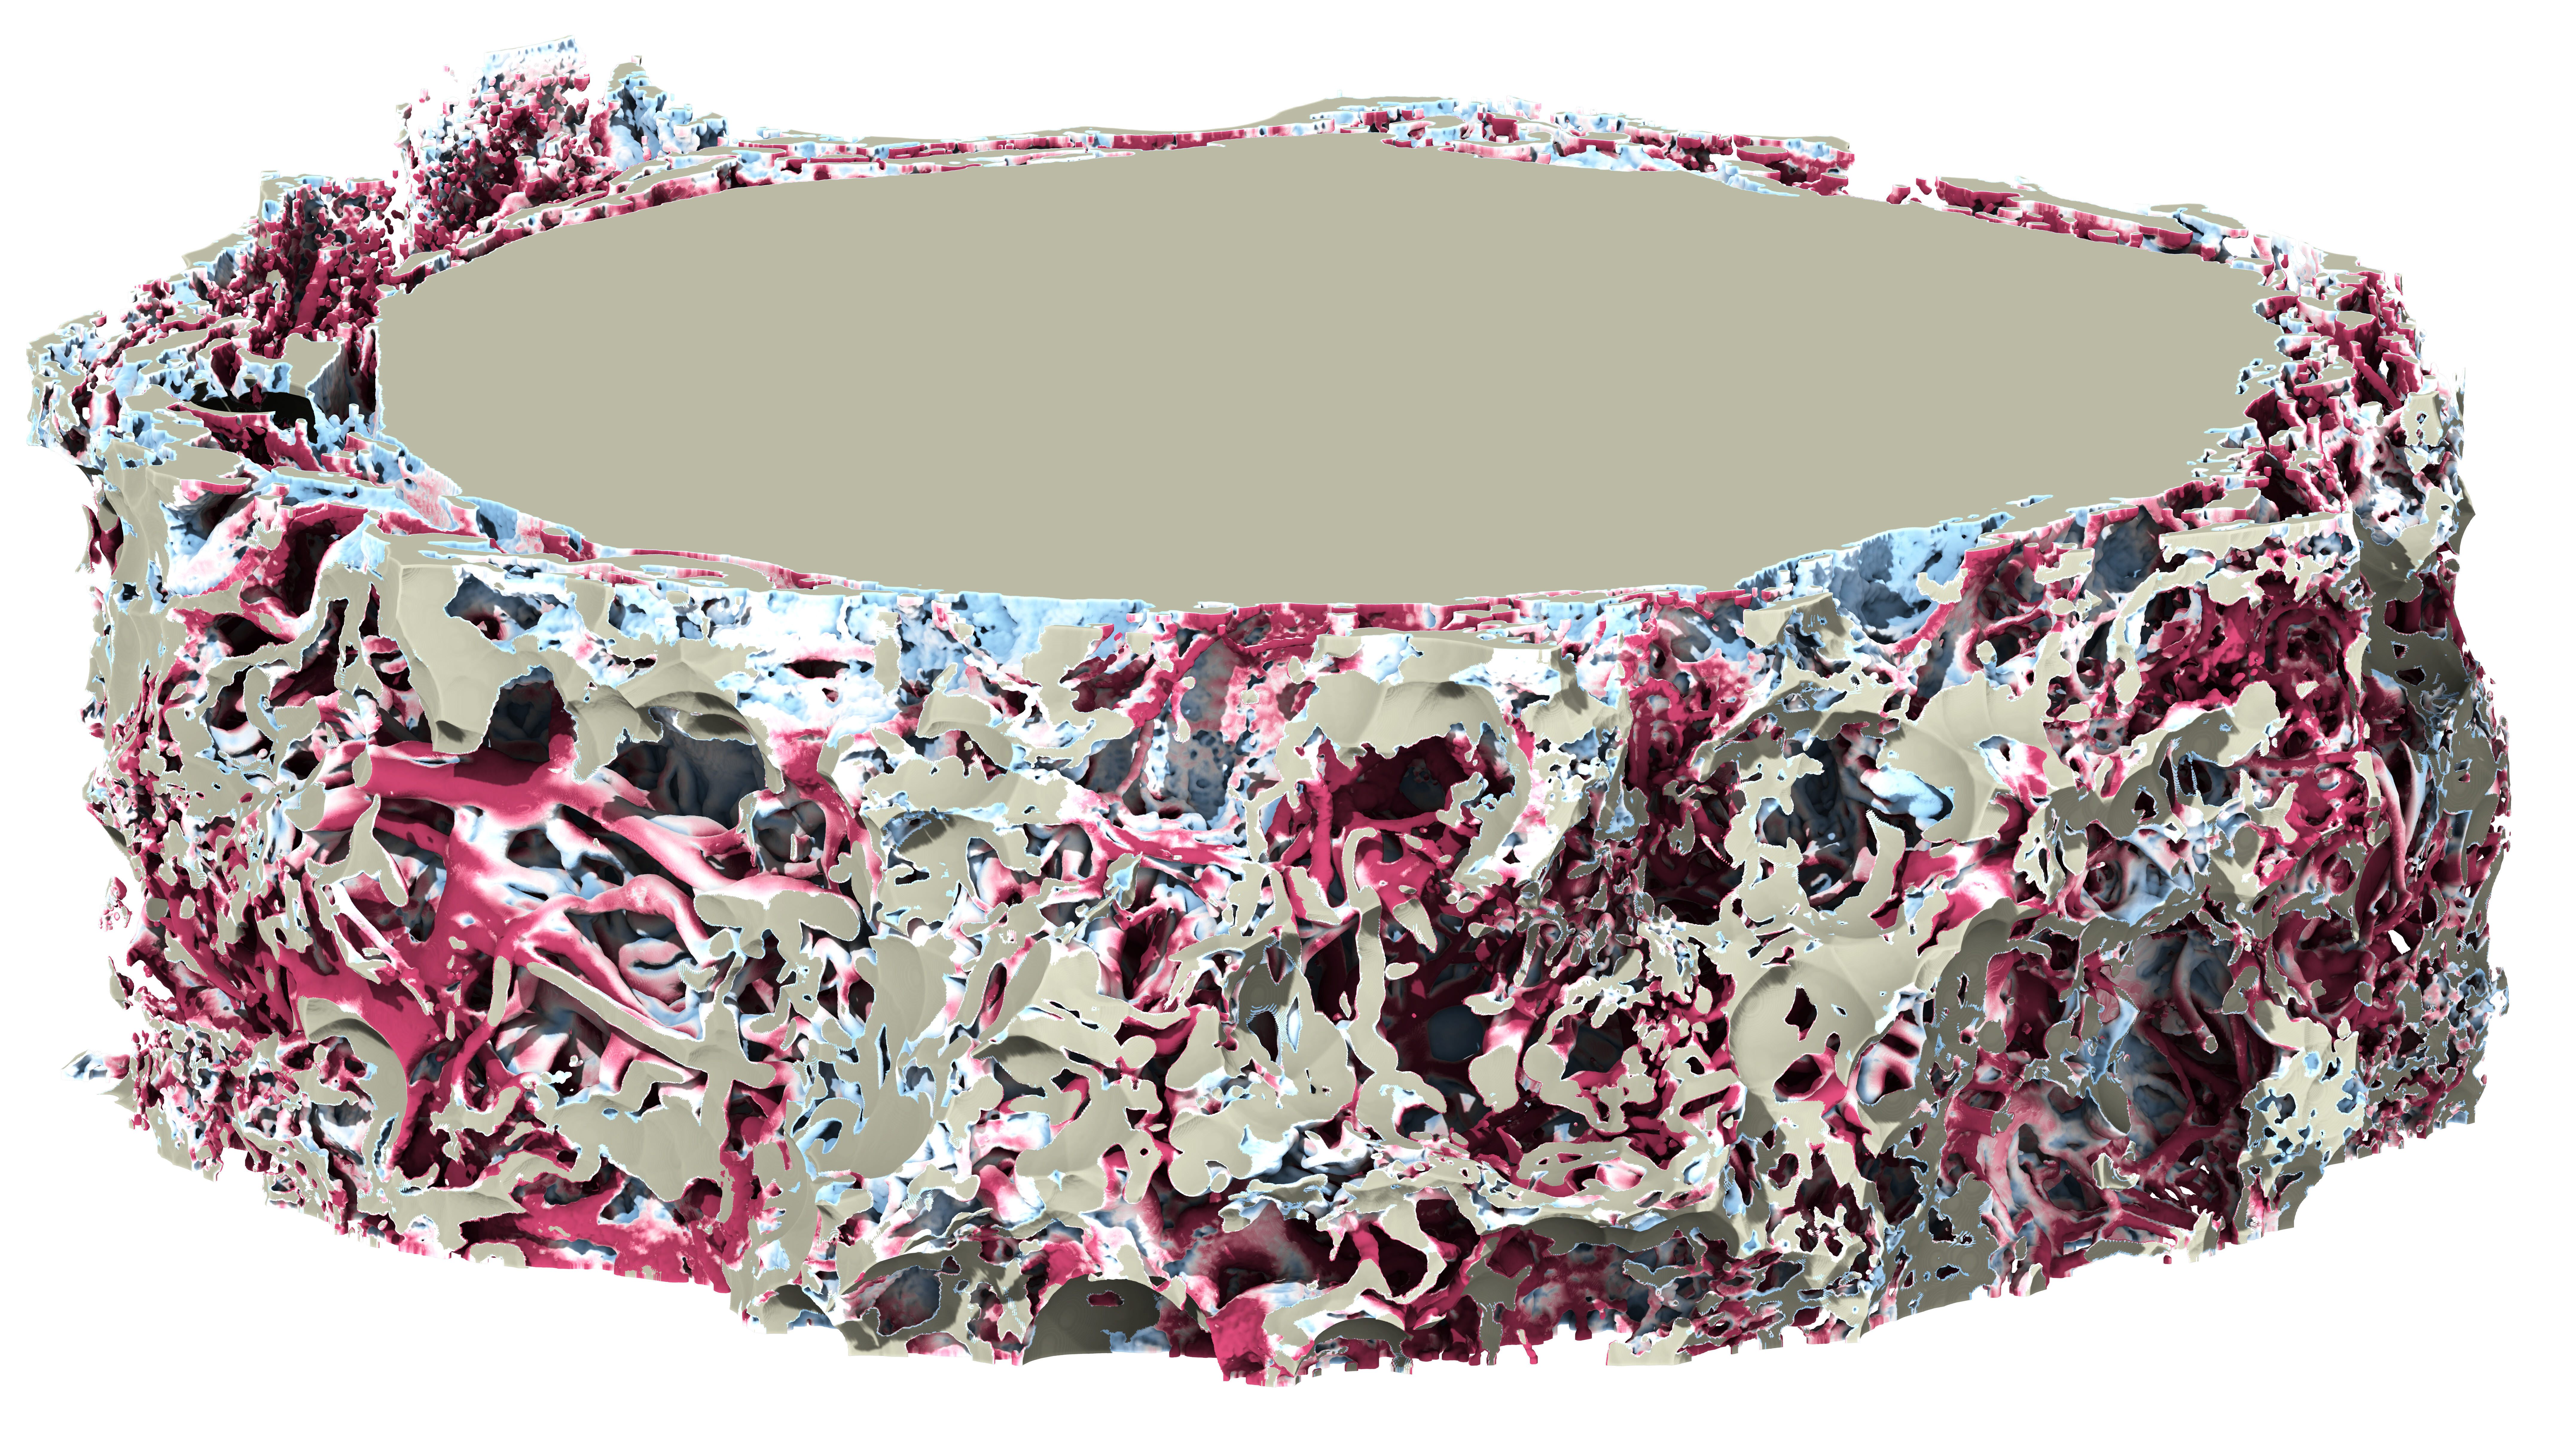
\includegraphics[width=1\columnwidth]{images/homeostasis-log-v2.jpg}
		\caption{Large-scale in-silico investigation of homeostasis in the subarachnoid space of the human optic nerve [Rossinelli et al. 2023, in-preparation]. Homeostasis is directly related with the interaction between the cerebrospinal fluid flow (not shown here) and the meningeal surface. Blue denotes poor levels of homeostasis, whereas red denotes sufficient material exchange between fluid and structure.}
		\label{fig:optical_nerve_3D}
	\end{figure}
	
	Whilst scientific visualization might be perceived as primitive, it is nonetheless an essential tool with which to reveal insight from 3D data sets, as demonstrated in Figure \ref{fig:closeup} which was provided by \cite{high_quality_2} and \cite{slice}. To better understand signals, we calculate how light is transported within the data volume. Massive amounts of light rays are cast from the sky, from every directions. To obtain accurate results in reasonable time on Terabytes, or hundreds of Gigabytes of data, the associated computational workload must be carried out at high fraction of nominal peak of the underlying computational infrastructure.
	
	\begin{figure}
		\centering
		\includegraphics[height=0.37\columnwidth]{images/multiscale-registration-lores.jpg}
		\includegraphics[height=0.37\columnwidth]{images/closeup-D.jpg}
		\caption{Two different types of data analysis, on the same data set. Gray-scale slice of the subarachnoid space of the optic nerve (left) and close-up view of the subarachnoid space of the optic nerve (right). The signal is the same, but the two data processing approaches lead to qualitative different insight.}
		\label{fig:closeup}
	\end{figure}
	
	For the purpose of this work, radiative transfer governing the transport of light is limited so as to only consider light attenuation, by assigning a linear mapping from grayscale signal intensities to light absorption values. 
	
	Herein high-performance high-accuracy rotations of volumetric images are relied upon to align data with arbitrary directions of rays that are cast. 
	Although 3D rotations are employed herein for a specific purpose, we emphasize that such operations are ubiquitous across most disciplines relating to imaging.
	For example, rotations are fundamental in multi-modal imaging, to align different signals of the same specimen under rigid body transformations.  
	%Computerized Tomography (CT) scans and Positron Emission Tomography (PET) scans. While the former provides detailed structural images, the latter measures molecular activity and we can use image rotation to combine the two to capture other aspects of the structure. 
	Typically solved in a supervised learning context, data augmentation for machine vision tasks is another example where fast but accurate 3D rotations are essential.
	
	\section{Prior Work and Methods}	
	This work seeks to find compromises between algorithmic efficiency, which lower the number of required operations for a certain task, and high-throughput processing schemes, which maximizes the number of operations that can be performed over a certain period of time. More often than not, algorithmic efficiency and execution efficiency are conflicting goals. Careful considerations are hence required to successfully combine 
	the two in order to aggressively decrease execution time.
	
	
	\subsection{Factoring 3D Rotations into 2D Rotations}
	We rely on Euler angles to represent arbitrary 3D rotations. To apply a rotation on a volumetric dataset we therefore perform a series of 2D rotations on the volumetric signal, in different directions. Each 2D rotation is carried out to each slice of the volume, independently. While such approach would already expose thread-level parallelism, abundantly available on CPUs and GPUs, it would lead to data access inefficiencies due to lack of spatial locality (e.g., while performing rotations on the $XZ$-plane). This issue is mitigated with global data transpositions, thereby ensuring that 2D rotations are always performed on the fastest varying indices of the dataset. While the cost of data transposition is not negligible, the underlying computational patterns expose enough regularity to be performed very efficiently on contemporary hardware including some of the latest ASICs \cite{neuralengine}.
	
	
	
	
	We rely on the work of Unser \cite{main_article} to implement 2D image rotations by resampling the translation of 1D signal (as shown in Figure \ref{fig:chinese_rotation}), independently for each line of each slice. This allows us to express rotations with schemes that expose both instruction-level and data-level parallelism, while maintaining close-to-ideal spatiotemporal locality.
	
	% \subsection{Manipulating frequency components of an image}
	% The raw imaging data that we acquire provides us with information regarding its frequency components at multiple scales. The manipulation of these components in the frequency domain allows us to build a 1D convolution filter that we will use to shift the original signal with by a fractional amount. As we see in section 2 we need to be careful when shifting a signal by non-integer values as the frequency components need to be handled correctly.
	% At first we will create a convolution filter with the Discrete Time Fourier Transform of a cosine function in an interval $[-M,M]$ . Defining the function in the Fourier space allows us to fine tune the filter to have a better control over the smoothing effect that will occur when we shift by fractional amounts. The filter is small compared to the original signal. Finally we will perform direct convolution of the signal with the computed filter.
	
	
	
	% While in the paper that this project takes inspiration from, the high frequency components that result from shifting by a fractional amount are simply cut-off 
	% The report will be covering different aspects of the Fourier domain and of convolution in section 2, while the exact implementation of the convolution will be handled in section 3.
	% Our code will generate algorithmically efficient schemes in order to ensure high performance on a. 
	
	%	\subsection{2D rotations as 1D translations}
	%	Starting from a reference paper \cite{main_article} we found that 2D rotations can be simply expressed as 1D translations by modifying the traditional rotation matrix.
	
	
	%	What is the contribution in the project: How to create a filter, show implementation and maybe study the numerical performance
	%	Accurate rotation requires the use of some fundamental signal processing concepts: Fourier domain and convolution of a signal with a filter. Filters are necessary in this work for their simplicity and ease of computational complexity. It will be shown how to create a filter to use as kernel for convolution with the original signal to rotate by fractional amounts. Something that is quite difficult to do accurately with traditional methods of interpolation for example. 	
	
	
	% Grafici fatti per interpolatzione lineare e cubica di un cos function.
	% \subsection{Interpolation}
	% Sampled version of our translated signal is:
	% \begin{equation}
		% 	(T_\Delta s)[k] = \sum_{l \in Z}^{} c(l)\varphi(k - \Delta - l)
		% \end{equation}
	% Where $\varphi$ is our generating function.
	% \subsubsection{Linear Interpolation}
	% With linear interpolation we want to estimate the coordinates of a point from a given number of samples. 
	
	% Linear interpolation model of function sin(x) with $N = 2$:
	% \begin{equation}
		% 	\beta^1(x) = 
		% 	\begin{cases}
			% 		1 - |x|, & |x| < 1    \\
			% 		0,       & otherwise, 
			% 	\end{cases}
		% \end{equation}
	% \begin{center}
		% 	\includegraphics{"images/linear_interpolation_example.pdf"}
		% \end{center}
	
	% Cubic spline interpolation model of function sin(x) with $N=4$:
	% \begin{equation}
		% 	\beta^3(x) = 
		% 	\begin{cases}
			% 		2/3 - |x|^2 + |x|^3/2, & 0 \leq|x| < 1  \\
			% 		(2-|x|)^3/6,           & 1 \leq |x| < 2 \\
			% 		0,                     & 2 \leq |x|     
			% 	\end{cases}
		% \end{equation} \cite{main_article}
	
	% \begin{center}
		% 	\includegraphics{"images/cubic_interpolation_example.pdf"}
		% \end{center}
	
	% Standard 2-D interpolation formula for computing the value of the image at location $(x,y)$
	% \begin{equation}
		% 	s(x,y) = \sum_{k = k_0}^{k_0+L-1}\sum_{l=l_0}^{l_0+L-1} c(k,l)\varphi(x-k)\varphi(y-l)
		% \end{equation}
	
	
	
	% 		As stated in the introduction we will take advantage of the fact that a 2D rotation can be expressed as a 1D translation which we reference from this article \cite{main_article}. 
	% 		In the case of the article the authors propose the use of different convolution-based interpolation schemes such as polynomial splines of degree $n$, cubic spline, etc. to translate a 1D signal. These operations are inherently global, which is not particularly effective since translation is a fundamentally local operation.
	% 		In our case however we will perform local direct convolutions on the original signal with a filter, whose frequency components we manipulate in the frequency domain.
	% %		In \cite{main_article} these translations are performed by downsampling the image before performing B-spline interpolations to shift the signal. The interpolation is done to flatten out the spurious oscillations that are due to high order 
	% 		 To create our own convolution filter in the frequency domain we will start with the Discrete Time Fourier Transform of a cosine function in an interval $[-M,M]$ . Defining the function in the Fourier space allows us to fine tune the filter to have a better control over the smoothing effect that will occur when we shift by fractional amounts. The filter is small compared to the original signal. Finally we will perform direct convolution of the signal with the computed filter.
	
	\subsection{Factoring 2D Rotations in 1D translations}
	
	Unser et al. \cite{main_article} have shown that a rotation transformation,
	\begin{equation*}
		R(\theta) = 
		\begin{pmatrix}
			\cos\theta & -\sin\theta\\
			\sin\theta & \cos\theta
		\end{pmatrix},
	\end{equation*}
	can be factored into three matrices each of which represents a shearing of the image in a cardinal direction:
	\begin{equation}\label{3_translations}
		R(\theta) = 
		\begin{pmatrix}
			\cos\theta & -\sin\theta\\
			\sin\theta & \cos\theta
		\end{pmatrix}
		=
		\begin{pmatrix}
			1 & -\tan\theta/2\\
			0 & 1
		\end{pmatrix}
		\cdot
		\begin{pmatrix}
			1 & 0\\
			\sin\theta & 1
		\end{pmatrix}
		\cdot
		\begin{pmatrix}
			1 & -\tan\theta/2\\
			0 & 1
		\end{pmatrix}.
	\end{equation} 
	\begin{figure}
		\centering
		\includegraphics[width=0.5\columnwidth]{images/unser_rotation.png}
		\caption{Rotation of an image is carried out by cascading translation operations, courtesy of Unser et al. \cite{main_article}.}
		\label{fig:chinese_rotation}
	\end{figure}
	The intermediate results within the factorization are shown in Figure \ref{fig:chinese_rotation}.
	A remarkable property of the shear matrices is that they involve no scaling: the diagonal entries of the matrices are the unity. This means that no frequencies are created or lost, as upsampling and downsampling are avoided, respectively.
	
	The first matrix shears the image in the $x$ direction by $\Delta_x = -y\cdot \tan(\theta/2)$, the second matrix shears the image in the $y$ direction by $\Delta_y = x \cdot \sin(\theta)$ and the last matrix shears the image again in the $x$ direction by $\Delta_x$ , as illustrated in (\ref{fig:chinese_rotation}).
	
	We use data transpositions to ensure that 1D translations are performed only on the fastest varying indices of a given line thereby enforcing ideal spatial locality during this computational stage. Therefore we temporarily swap rows with columns, whenever needed.
	
	This work is focused on the design and implementation of computational compact schemes that resample 1D signals translated by a (constant) fraction of the sampling distance. 
	
	
	\subsection {Resampling Translation with Finite Impulse Response (FIR) Filters}
	In the work of Unser et al. \cite{main_article}, translation of each row (resp. each column) is carried out by evaluating an interpolation scheme:
	\begin{equation}
		f(x-h) \approx \sum_ic_i\phi(x-h - x_i),
	\end{equation}
	where $h$ is the translation parameter (also called ``shift'' in the present document), $f$ is the input signal, $\phi$ is the reconstruction kernel, and $c_i$ are the interpolating coefficients.	
	
	As reconstruction kernel, Unser et al. \cite{main_article} consider B-splines of order 1, 3, 7.
	Except for the linear B-spline, which is interpolating by design, higher order B-splines are non-interpolating (in fact they are low-pass filters), and thus one has to solve a system of interpolating equations:
	\begin{equation}
		f_i = f(x_i) = \sum_jc_j\phi(x_i - x_j),
	\end{equation}
	with $x_i = i$. The system size is the size of the input signal, and the latter can be in the order of ten thousand samples. Inverting a linear system of equations $Ax = b$ of such sizes may incur non-negligible computational costs.
	
	In their work, Unser et al. \cite{main_article} organize the computational workload of translating a 1D signal in two separate stages: computing the interpolating coefficients, and resample translated signals by evaluating the interpolation scheme at the sample locations.
	
	When B-splines are used as reconstruction kernels, the system can be inverted very efficiently \cite{unser1993b} by cascading a few infinite impulse response (IIR) filters.
	Despite such algorithmic advantages, the linear system remains global. This is somewhat disappointing: the resampled translation of the signal at a given point will ``see'' only a limited set of adjacent points. 
	
	If $\phi$ has compact support, why then try to solve a global system ? This issue motivates the research on alternative computational schemes that are completely local.
	Herein we opt to resampling translated 1D signals by carrying out direct convolution with filters of compact support, and avoiding solving global system of equations in the first place.     The type of filters sought herein are finite impulse response (FIR). 
	Direct convolution of a FIR filter $h$ to an input signal $x$ reads:
	\begin{equation}
		y(n) = \sum_{k=A}^{B}h(k)x(n-k)=(h*g)(n).
		\label{direct_convolution_equation}
	\end{equation}
	
	\begin{figure}
		\centering
		\includegraphics[width=0.4\columnwidth]{images/ifft_filter_m_2_25_shift.png}
		\caption{Example of a FIR filter $z(t)$ that we will create.}
		\label{fig:final_filter}
	\end{figure}
	
	While direct filtering (carried out by direct convolution) is generally seen as inefficient, it can be carried out at outstanding performance if the filter is reasonably small, when carefully implemented on contemporary microarchitectures. Firstly,
	direct convolution maps independent workloads to each output entry. When carefully implemented, it exposes instruction-level parallelism which can be discovered at runtime by superscalar microarchitectures featuring out-of-order execution. Secondly, the regular access pattern of direct convolution allows to expose data-level parallelism in the form of single-instruction multiple-data operations. Thirdly, the abundance of independent workload can be leveraged by thread-level parallelism.
	In addition, direct convolution with small filters may bring crucial advantages on specific computing architectures such as digital signal controllers, or the A100 GPU, where one can use the tensor cores to carry out a block-sparse form of the direct convolution in single precision \cite{a100whitepaper}.
	
	\textbf{Our goal is therefore to design a FIR filter of relatively compact support (e.g., 20 - 40  coefficients) that will be used to shift a signal by any real value by  direct convolution, while also allowing us to outperform both in terms of accuracy and efficiency the approach proposed by Unser et al. \cite{main_article}.}
	
	
	The technical strategy we embrace is as follows: 
	\begin{itemize}
		\item We design our filter in Fourier space for any frequency in $[-\pi/2, +\pi/2[$ (DTFT space).
		\item We digitize it for the number of coefficients we desire (DFT space). 
		\item We obtain the filter coefficients in the time domain by performing an inverse DFT (IDFT).
	\end{itemize}
	We would like to mention that the coefficients of a FIR filter is also its impulse response.
	
	The target filter, exemplified in Figure \ref{fig:final_filter}, is obtained by cascading two filters:
	\begin{itemize}
		\item $H(\omega)$, the filter to carries out a spectral shift of the signal, thus leveraging the perfect interpolation property available in Fourier space.
		\item $F(\omega)$ filter mitigates the Gibbs phenomenon, arising from the truncation of the Fourier series to a finite size. This issue is more apparent in smaller filters than larger ones.
	\end{itemize}
	
	\subsection{Design of the Translation Filter $H(\omega)$}
	
	For a digital signal of infinite length,  an arbitrary shift $\delta$ applied on the signal can represented exactly with the transfer function:
	\begin{equation}
		H(\omega) = e^{-i\delta\omega}.
	\end{equation}
	%    Here we derive 
	% %In signal processing working in the frequency domain has a great advantage since any function that is expressed in this way can be reconstructed completely via an inverse process, with no loss of information.\cite{image_book}
	% We use the Discrete Fourier Transform (DFT) of a function $g(x)$ to analyze its frequencies, as follows:
	% \begin{equation}
		% 	F_m = \displaystyle\sum_{k=0}^{N-1}f_ke^{-i \frac{2\pi}{N}km}
		% \end{equation}
	% In this project the above equation will not be used since the filter that is going to be defined in one of the next chapters, will be created directly in the Fourier domain. Nevertheless it is useful to show the definition since it is the Inverse Discrete Fourier Transform that will be used to reconstruct the filter in the time domain:
	% \begin{equation}
		% 	f_n = \frac{1}{N}\displaystyle\sum_{k=0}^{N-1}F_ke^{i \frac{2\pi}{N}kn}
		% \end{equation}
	The (forward) DFT of a digital 1D signal $f$ reads:
	\begin{equation*}
		F_m = \displaystyle\sum_{k=0}^{N-1}f[k]e^{-i \frac{2\pi}{N} km},
	\end{equation*}
	where $N$ the number of samples and $m$ the wave number.	
	We approximate ``$f[k - \delta]$'' where $\delta$ is the amount we want to shift:
	\begin{align*}
		Z_m &= \displaystyle\sum_{k=0}^{N-1}f[k - \delta]e^{-i \frac{2\pi}{N} km},\\
		% sbagliata questa!!! &= \displaystyle\sum_{r = 0 - \delta}^{N-1-\delta}f[r]e^{-i \frac{2\pi}{N} km}, r = k - \delta \\
		&= \displaystyle\sum_{r= -\delta}^{N-1 - \delta}f[r]e^{-i \frac{2\pi}{N} (r + \delta)m}.
	\end{align*}
	We take the common term outside the summation:
	\begin{align*}
		%non c'e' bisogno di questa!! Z_m &= \displaystyle\sum_{r= -\delta}^{N-1 - \delta}f[r]e^{-i \frac{2\pi}{N} rm}e^{-i \frac{2\pi}{N}  \delta m}\\
		Z_m &= e^{-i \frac{2\pi}{N}  \delta m} \displaystyle\sum_{r= -\delta}^{N-1 - \delta}f[r]e^{-i \frac{2\pi}{N} rm},\\
		&= e^{-i \frac{2\pi}{N}  \delta m} \displaystyle\sum_{k=0}^{N-1}f[k]e^{-i \frac{2\pi}{N} km}.
	\end{align*}
	%\begin{equation}
	%	Z_m = e^{-i \frac{2\pi}{N}  \delta m} F_m = H_m \cdot F_m \label{shift_equation}
	%\end{equation}
	Therefore, the transfer function of the shift filter in the DFT space reads:
	\begin{equation}
		H(\omega_m) = \frac{Z(\omega_m)}{F(\omega_m)} = e^{-i  \delta \omega_m  }, 
	\end{equation}with $\omega_m = \frac{2 \pi}{N}m$.
	% If we want to express this transfer function as a DTFT then our transfer function $H(\omega)$ would look more like this:
	% \begin{equation}
		%     H(\omega) = \sum_{-\infty}^{+\infty} e^{-i\omega \delta}
		% \end{equation}
	
	% \paragraph{Interpretation of the Discrete Frequencies}
	The last equation works well for any integer shifts that we want to perform on our signal but for any fractional amount we encounter some problems with the use of the correct frequency indexes. The small diagram in Figure \ref{fig:wavenum_plot} depicts this problem on the left and our solution on the right. 
	% We first take into consideration the positive frequencies from $w=0$ to $w=\pi$ then we follow up with the negative frequencies...
	%\begin{figure}
	%	\centering
	%	\includegraphics[width=0.25\columnwidth]{images/freq_index_circle.png}
	%	\caption{Two different enumerations of the discrete frequencies Complex unit circle diagram which depicts two method of traversing the circle's perimeter.}
	%   \label{fig:freq_circle}
	%\end{figure
		%	And we can see that from $N/2$ we start getting negative values for the  magnitutde of each frequency. These negative values correspond the the complex conjugate of each frequency.
		% As stated in equation \ref{shift_equation} we multiply each sample by its corresponding phase, which is based on the frequency number $m$.
		We need to take into consideration the negative frequency indexes for fractional shifts in order to maintain the Hermitian symmetry of the spectrum of real-valued signals. As such we define a function called $\mathrm{wave\_}n$ that maps indices to the correct wave number:
		\begin{equation}
			\mathrm{wave\_}n(m) = (m + \lfloor N/2 \rfloor ) \bmod N - \lfloor N/2 \rfloor
		\end{equation}
		This equation will assign each frequency it's correct index (Figure \ref{fig:wavenum_plot}).
		\begin{figure}
			\centering
			\hfill
			\parbox{0.4\linewidth}{\centering
				\includegraphics[width=\linewidth]{images/freq_index_circle.png}
			}\hfill
			\parbox{0.48\linewidth}{\centering
				\includegraphics[width=\linewidth]{images/wavenum_40.png}
			}\hfill
			\caption{Different enumeration of the discrete frequencies (left), and correct enumeration for translating signals (right), function on $n=40$ samples.}
			\label{fig:wavenum_plot}
		\end{figure}
		%	Modify original equation to use wavenum.
		%	\begin{equation*}
			%		H_m = e^{-i \frac{2\pi}{N}  \delta wave\_n(m)}
			%	\end{equation*}
		%	\begin{equation}\label{phase_shift_equation}
			%		Z_m = H_m \cdot F_m 
			%	\end{equation}	
		
		% $DFT^{-1} (\{H(\omega_{i}) F(\omega_{i})\}_i)$
		
		
		%	Afterwards we implemented a simple version of the inverse Fourier transform, which give us our signal in the time domain. Before returning the result however we need to perform the equivalent of numpy's fftshift function to have the filter values centered. This whole operation can be done in serial and with no real optimization of the code since the kernel size will always be much smaller than the input signal and as such will no be computationally expensive.
		
		\subsection{Integer Shifts} 
		Any shift $s$ on the input signal can be decomposed into integral and fractional parts  $k = \lfloor s \rfloor $, $\delta = s - \lfloor s \rfloor$, respectively.
		Shifting a signal by $k$ is a trivial operation, as it boils down to moving the array by $k$ entries. Therefore, if the shift does not have a fractional component then we skip the convolution with the filter entirely.
		
		%Now that the fractional part of the shift has been taken care of we need to shift the %signal by the integer value.
		%To shift a signal by an integer amount we used the C function \textsl{memcpy} to copy the values of the original array to a resulting array but at a different position, which is defined by the integer shift. We chose \textsl{memcpy} instead of just moving the values inside the same array with \textsl{memmove} since \textsl{memcpy} is designed to be the fastest library routine to copy data from memory to memory.
		
		%\newpage
		%	Here is some pseudo-code that explain what is being done to our original filter:
		%	\begin{algorithm}
			%		\caption{Filter shift}\label{alg:cap}
			%		Write convolution algorithm defined with compiler explorer
			%	\end{algorithm}
		%	
		
		% \iffalse
		
		
		% \begin{figure}
			% 	\centering
			% 	\includegraphics[width=0.5\columnwidth]{images/box_shifted_delta10_1_n50.png}
			% 	\caption{Shifted function by $\delta=10.5$}
			% \end{figure}
		
		% \subsection{Lanczos Filter and FIR}
		% To alleviate the problems that arise when shifting a signal by a fractional amount we can use a filter $L$ that is convoluted with the shifted signal.
		
		% \begin{align*}
			% 	L_m &= \frac{\sin(a)}{a},\\
			% 	a &= \frac{2\pi wave\_n(m)}{N}
			% \end{align*}
		
		% Apply lanczos filter to fractional shift to smooth the result.
		
		% \begin{equation*}
			% 	Z_m = L_m \cdot H_m \cdot G_m
			% \end{equation*}
		
		% \begin{figure}[h]
			% 	\centering
			% 	\includegraphics[width=0.5\columnwidth]{images/box_shifted_lanczos_delta10_1_n50.png}
			% 	\caption{Shifted function by $\delta=10.5$ with lanczos filter applied (red), no filter(blue).}
			% \end{figure}
		
		% \fi
		
		\subsection{Design of the Smoothing Filter $F(\omega)$}
		For a digital signal of infinite length,  an arbitrary shift $\delta$ applied on the signal can represented exactly with the transfer function $H(\omega) = e^{-i\delta\omega}$. 
		When dealing with finite signals of $N$ samples, however, the frequency spectrum is sampled into $N$ frequency bins.  In such settings, any $\delta$ that is not a multiple of $1 / N$ would lead to spurious oscillation  due to the Gibbs phenomenon. The strongest spurious oscillations are obtained for $\delta = 0.5$.
		
		The goal of the smoothing filter is therefore to attenuate the oscillations that occur.
		We rely on an approach inspired from the Lanczos smoothing kernel \cite{hamming1998digital}.
		While the Lanczos analog filter in the time domain is a tiny box covering 4 samples, our analog filter $g$ is the Dirac function, mollified over $2M$ samples:
		\begin{equation}\label{filter_formula}
			g(t) = \frac{1}{2} + \frac{1}{2} \cos(\frac{\pi t}{M}),
		\end{equation}
		with $M$ chosen between $1.5$ and $3$. 
		Along the same approach of Lanczos smoothing, we perform a Continuous Fourier Transform (CFT) of our filter and resample it to obtain its Discrete Fourier Transform (DFT) representation, and combine it with the DFT version of $H(\omega)$.
		The Continuous Fourier transform (CFT) on the cosine part of $g$ reads:
		\begin{equation}
			F(\omega) = \int_{-M}^{M} \cos(\frac{\pi}{M}t)\mathrm{e}^{-\mathrm{i}\omega t}\mathrm{d}t.
		\end{equation}
		
		%This is because in DTFT we have access to any angular speed
		%	this section we propose an example of the smoothing filter.
		This equation allows us to define our CFT in an interval $M$, that we choose based on the fractional amount we want to shift. The parameter M is useful for us to fine tune the filter and choose how big of a smoothing effect we want:
		\begin{equation}\label{filter_formula}
			F(\omega) = \frac{2M^2\omega \sin(M\omega)}{M^2\omega^2-\pi^2}.
		\end{equation}
		
		Using this function we can build filters of different M sizes(Figure \ref{fig:filters}).
		% Filters.
		\begin{figure}
			\centering
			\includegraphics[width=0.4\columnwidth]{images/filter_m_1.png} \hfill		\includegraphics[width=0.4\columnwidth]{images/filter_m_1_5.png} \\
			\parbox{0.4\columnwidth}{\centering $F(\omega)$ with $M = 1$} \hfill
			\parbox{0.4\columnwidth}{\centering $F(\omega)$ with $M = 1.5$}
			\centering
			\includegraphics[width=0.4\columnwidth]{images/filter_m_2_40.png} \hfill		\includegraphics[width=0.4\columnwidth]{images/filter_m_3.png} \\
			\parbox{0.4\columnwidth}{\centering $F(\omega)$ with $M = 2$} \hfill
			\parbox{0.4\columnwidth}{\centering $F(\omega)$ with $M = 3$}
			\caption{Compact schemes of different M for local computation.}
			\label{fig:filters}
		\end{figure}
		%
		
		%	In figure \ref{filters} we can see the general shape of the function for each M and the number of samples it will use for convolution. 
		%	It does not however give us a good idea on how it is going to modify the signal. In the next figure we can see the same filters but in the time domain.
		% Filters. % impulse reposne
		
		For better accuracy we generally choose our interval M to be small when we have a small fractional shift and big when we have a shift that gets closer to $0.5$. We can write a simple expression that defines M in respect to the fractional shift $x$ to be:
		
		
		% Tenere?
		\begin{equation*}
			M = 
			\begin{cases}
				1.5 & \text{if}~ 0.1 < x < 0.25\\
				2 & \text{if}~ 0.3 < x < 0.5
			\end{cases}
		\end{equation*}
		
		With some experimenting we found that the filter with $M=3/2$ is a good compromise between eliminating the oscillations and translating the signal as accurate as possible.
		
		We will create one of size $40$ with $M=2$. We then follow equation \eqref{filter_formula}, while also paying attention to evaluating the limit when $\omega=\frac{\pi}{M}$ or $\omega=-\frac{\pi}{M}$. This results in $F(\omega)$ which we plot in Figure \ref{fig:h_f_filters}.
		
		Now let us say that the fractional amount to shift is $0.1234$. We then multiply our smoothing filter $F(\omega)$ by our shift filter $H(\omega)$ (Figure \ref{fig:h_f_filters}), which gives us $Z(\omega)$.
		
		Finally, we carry out the Inverse Discrete Fourier Transform (IDFT) of the digitized $H(\omega)F(\omega)$ to obtain the coefficients of the target FIR filter in the time domain $z(t)$, as already depicted in Figure \ref{fig:final_filter}.
		
		
		\begin{figure}
			\centering
			\includegraphics[height=0.25\columnwidth]{images/h_filter.png}\hspace*{0.1\columnwidth}
			\includegraphics[height=0.25\columnwidth]{images/filter_m_2.png}\\
			\parbox{0.4\columnwidth}{\centering $H(\omega)$ Filter with $M=2$}\hspace*{0.1\columnwidth}
			\parbox{0.4\columnwidth}{\centering $F(\omega)$ Shift filter with $\delta=0.1234$}
			\caption{The two filters $H(\omega)$ and $F(\omega)$.}
			\label{fig:h_f_filters}
		\end{figure}
		
		
		
		\section{Software Implementation Details}
		
		%		\begin{itemize}
			%			\item creazione filtro e spiegare perche IFT invece di ifft
			%			\item perche direct convolution invece di fft
			%			\item code generation at compile time with python script
			%			\item piccola spiegazione su SIMD e metodo di convoluzione per facilitare la vettorizzazione dell'assembly code
			%		\end{itemize}
		
		%We chose a bottom-up approach for this project since we saw that the implementation steps were well suited for it. 
		%We started with the fundamentals of signal processing by exploring the Fourier Transform and its properties to build our shift filter. 
		
		
		The computational schemes discussed herein have the advantage of being data-independent.
		That is, they lead to opcode streams that contain no branching instructions that depends on the input data (except for the input and filter lengths).
		This provides two key advantages.
		Firstly, it allows us to benefit from static performance analysis.
		Secondly, the synthesis of C kernels can be straightforwardly automated in a programming language with a higher abstraction.
		
		In our case C kernels are generated by a python script executed at compile time by Makefile. The only parameter we define is the desired filter size. The script will generate a header and source file in C implementing the direct convolution.
		
		%\subsection{Efficient implementation of direct convolution on x86 microarchitectures}
		To assess our one-dimensional direct convolution kernel, we use the {\it Godbolt Compiler Explorer} \cite{godbolt}. This tool allows us to assess how effectively instruction-level and data-level parallelism are exploited by the compiler at hand. As stated in the introduction, what we are looking for is a balance between algorithmic efficiency and execution efficiency, whereby increasing the number of instructions per cycle while lowering the number of operations. This is depicted in Figure \ref{fig:conv_assembly}, targeting two different microarchitectures. From the signature of the C kernel we note that the single instruction stream is aliased into multiple input pointers (shifted by consecutive entries). This is to direct the compiler to the full SIMDization of the compute kernel. On the right hand side of Figure \ref{fig:conv_assembly} we note how well the compiler can transform the computational scheme into AVX and AVX-512 instructions. The AVX-512 instruction stream is exceptionally compact, featuring 1.5 FLOP/instruction and thus able to attain 75\% of the nominal peak performance, when not memory-bound.
		
		\begin{figure}
			\centering
			\includegraphics[height=0.45\columnwidth]{images/normal_code.png}\hspace*{0.1\columnwidth}
			\includegraphics[height=0.45\columnwidth]{images/asm-listing.png}\\
			\caption{Static assessment with {\it Godbolt Compiler Explorer} of a direct convolution with an 8-coefficients filter on an arbitrary long digital signal. C kernel (left), successfully compiled for AVX2 enabled microarchitectures (right, top), and microarchitectures featuring AVX-512 SIMD instructions(right,bottom). }
			\label{fig:conv_assembly}
		\end{figure}
		
		\newpage
		\section{Results}
		\subsection{Results with 1D signals.}
		One-dimensional signals are the starting point of our tests and as such we chose the reversed unit step, a pretty aggressive signal to test (Figure \ref{fig:original_signal}). For a signal of $n=100$ samples the reversed unit step reads:
		\begin{equation*}
			g(x) = 
			\begin{cases}
				1	& \quad \text{if } x \leq \frac{n}{2}\\
				0	& \quad \text{otherwise}
			\end{cases}
		\end{equation*}
		\begin{figure}
			\centering
			\includegraphics[height=0.35\columnwidth]{images/original_signal.png}
			\includegraphics[height=0.35\columnwidth]{images/Results/M_1_small_shift.png}
			\caption{Original signal of size $n=100$ samples (Left) shifted by $\delta = 20.01$ with $M=1$(Right).}
			\label{fig:original_signal}
		\end{figure}
		
		By taking this signal and shifting it by $20.25$ we get a different result depending on the M chosen when creating the filter (Figure \ref{fig:results_1}).
		\begin{figure}
			\centering
			\includegraphics[width=0.4\columnwidth]{images/Results/M_1.png}\hspace*{0.2\columnwidth}
			\includegraphics[width=0.4\columnwidth]{images/Results/M_3_2.png}\\
			\parbox{0.4\columnwidth}{\centering $M = 1$}\hspace*{0.2\columnwidth}
			\parbox{0.4\columnwidth}{\centering $M = 1.5$}\\
			\centering
			\includegraphics[width=0.4\columnwidth]{images/Results/M_2.png}\hspace*{0.2\columnwidth}
			\includegraphics[width=0.4\columnwidth]{images/Results/M_3.png} \\
			\parbox{0.4\columnwidth}{\centering $M = 2$}\hspace*{0.2\columnwidth}
			\parbox{0.4\columnwidth}{\centering $M = 3$}
			\caption{Results of shifting the original signal $g(x)$ by $\delta=20.25$ with different sizes of $M$.}
			\label{fig:results_1}
		\end{figure}
		
		At first glance we can see that with $M=1$ we have  many oscillations present in the resulting signal and with $M=3$ the sharp features of the signal are completely smeared out. We can see though in the right of Figure \ref{fig:original_signal} that if we set $M=1$ and the fractional value is small, for example $0.01$ we have smaller oscillations and the output signal preserves well the features of the input signal.
		
		This result is attributed to the fact that the filter contains fewer oscillations as well. If we take a look at the filter defined for $M=1$ we can see that we have the strongest oscillations at $0.5$ (Figure \ref{fig:different_shifts_small_M}). 
		This is why for a fractional shift that gets closer to $0.5$ it could be beneficial to consider a larger value of M, such as $\frac{3}{2}$ or $2$, in order to damp out the oscillations.
		\begin{figure}
			\centering
			\includegraphics[width=0.33\columnwidth]{images/Results/M_1_filter_small_shift.png}
			\includegraphics[width=0.33\columnwidth]{images/Results/M_1_filter_big_shift.png}
			\includegraphics[width=0.33\columnwidth]{images/Results/M_2_filter_big_shift.png}
			\caption{Difference in oscillations with varying fractional shifts. $F(\omega)$ shifted by $0.01$ with $M=1$ (Left), $F(\omega)$ shifted by $0.5$ with $M=1$ (Middle) and $F(\omega)$ shifted by 0.5 with $M=2$(Right).}
			\label{fig:different_shifts_small_M}
		\end{figure}
		
		
		\section{Conclusion and Outlook}
		Information Technology (IT) has reached unprecedented rates of data acquisition and processing power. Data visualization is a crucial component in IT-assisted scientific inquiry, as it is employed both for gaining the initial insight from the acquired data and for the qualitative assessment of the results obtained by after computational modeling. High quality visualization relies on approximating how light interacts with volumetric structures, and such calculations can be simplified by leveraging 3D rotations. 
		
		The work presented herein is motivated by the need of processing of large volumes of data by leveraging contemporary distributed computing infrastructure. As such, it seeks to find computational patterns that leads to very high accuracy while executing exceptionally well on the latest computing microarchitectures.
		Following this direction, this report has elaborated the design and application of relatively small filters that translate large volumetric datasets to accurately rotate them in Euclidean space. Our approach implements 3D rotations by shifting the ``1D lines'' of the dataset by fractional amounts, and executes very well (i.e., at high fractions of the nominal peak) on contemporary CPU microarchitectures. Future work includes the extension of such filtering techniques on GPUs. Moreover, the choice of M for the filter could be chosen automatically based on the fractional amount we want to rotate.
		\newpage
		\bibliographystyle{plain}
		\bibliography{references}
		
		\section* {Supplementary Information}
		Numpy and Matplotlib were a huge help in visualizing the results of the Fourier Transform and of the shifts. These libraries were also useful for when we started writing code in C. Where we would output the binary result to a file and then read it and plot the result in python. There are a few plotting libraries for C like the gnuplot library but we felt that this was just the faster/easier solution.
		The whole project started out as a CMake and this was chosen mainly because of familiarity with this tool and teh ability to quickly setup an environment that would build the executable. However, towards the end used a plain Makefile to streamline the work. The added advantage of the makefile was to enable running a python script at compile time to create other files needed by the main target. 
		
		Jupyter Notebook was used extensively to test our method and quickly plot the results, while also documenting everything so that it would be easier to complete this report. Since we embraced a bottom-up approach we were able to re-use parts of the code to test some other aspect of the shift. We started with simple shifts of a 1D signal by an integer value which we then attempted to shift the same signal by a fractional amount. At this point some problems arose with the usage of the correct frequency index but in code was easily implemented it with a basic method. The source code of this project is available at: \url{https://github.com/DylanReidRamelli/Bachelor-Project-2023}.
		The tools that were used: MakeFile, CMake, Jupyter Notebook and some built-in libraries of C and Python like numpy and matplotlib.
		\section* {Acknowledgments}
		% Without taking credit
		% Is accredited,
		% Laying no claim
		% Is acclaimed
		% And, because he does not compete,
		% Finds peaceful competence.
		
		I would like to express my deepest appreciation to Dr Diego Rossinelli without whom this endeavour would have been impossible to complete. Next I would like to express my deepest gratitude to Dr Patrick Zulian for his belief in my ability to complete such a project and finally, my sincere gratitude to Prof Rolf Krause for his invaluable feedback and support.
		
		
	\end{document}